\noindent

\includegraphics[height=1.25cm]{images/pictograms/replication}
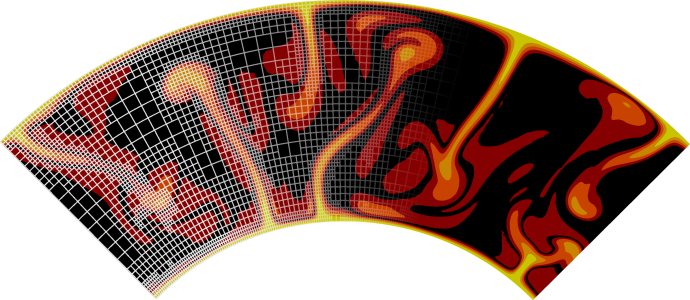
\includegraphics[height=1.25cm]{images/pictograms/aspect_logo}

\includegraphics[height=1.25cm]{images/pictograms/benchmark}

\includegraphics[height=1.25cm]{images/pictograms/under_construction}

\includegraphics[height=1.25cm]{images/pictograms/FEM}

\includegraphics[height=1.25cm]{images/pictograms/paraview}

%%%%%%%%%%%%%%%%%%%%%%%%%%%%%%%%%%%%%%%%%%%%%%%%%%%%%%%%%%%%%%%%%%%%%%%%%%%%%%%%%%%%%%%%%%%%%%%%%%%

\begin{flushright} {\tiny {\color{gray} \tt python\_codes/fieldstone\_160/text.tex}} \end{flushright}

%\lstinputlisting[language=bash,basicstyle=\small]{python_codes/template_keywords.key}

\par\noindent\rule{\textwidth}{0.4pt}

\begin{center}
\inpython
{\small Code: \url{https://github.com/cedrict/fieldstone/tree/master/python_codes/fieldstone_160}}
\end{center}

\par\noindent\rule{\textwidth}{0.4pt}

{\sl This stone was developed in collaboration with J.C. Afonso}. \index{contributors}{J.C. Afonso}

\par\noindent\rule{\textwidth}{0.4pt}


%%%%%%%%%%%%%%%%%%%%%%%%%%%%%%%%%%%%%%%%%%%%%%%%%%%%%%%%%%%%%%%%%%%%%%%%%%%%%%%%%%%%%%%%%%%%%%%%%%%


The domain is a Cartesian box of size $L_x=120~\si{\km}$, $L_y=100~\si{\km}$.
There are three materials in the domain:
\begin{itemize}
\item crust: $\rho_{c}=2300~\si{\kg\per\cubic\meter}$ and $\eta_{c}=10^{23}~\si{\pascal\second}$;
\item mantle: $\rho_{m}=3300~\si{\kg\per\cubic\meter}$ and $\eta_{m}=10^{21}~\si{\pascal\second}$;
\item weak zones: $\rho_{wz}=\rho_{c}$ and $\eta_{wz}=10^{-3}\eta_{c}$.
\end{itemize}
Free slip boundary conditions are imposed on all four sides. ${\bm Q}_2 \times Q_1$ 
(continuous pressure)
or ${\bm Q}_2\times P_{-1}$ (discontinuous pressure) elements are used.
The crust is 20~\si{\km} thick but is thickened (40~\si{\km} depth) in the middle 30~\si{\km}.
On each side we find weak zones as thick as the crust and 1~\si{\km} wide. 
The default resolution is set to 120$\times$100 elements.

The boundary conditions are such that the pressure can only be computed up to a constant (null space)
and it is therefore normalised by imposing that the average pressure at the surface is zero.

In all what follows temperature effects are discarded. A single Stokes solve is carried out, without any 
time stepping nor advection of the materials.

\begin{center}
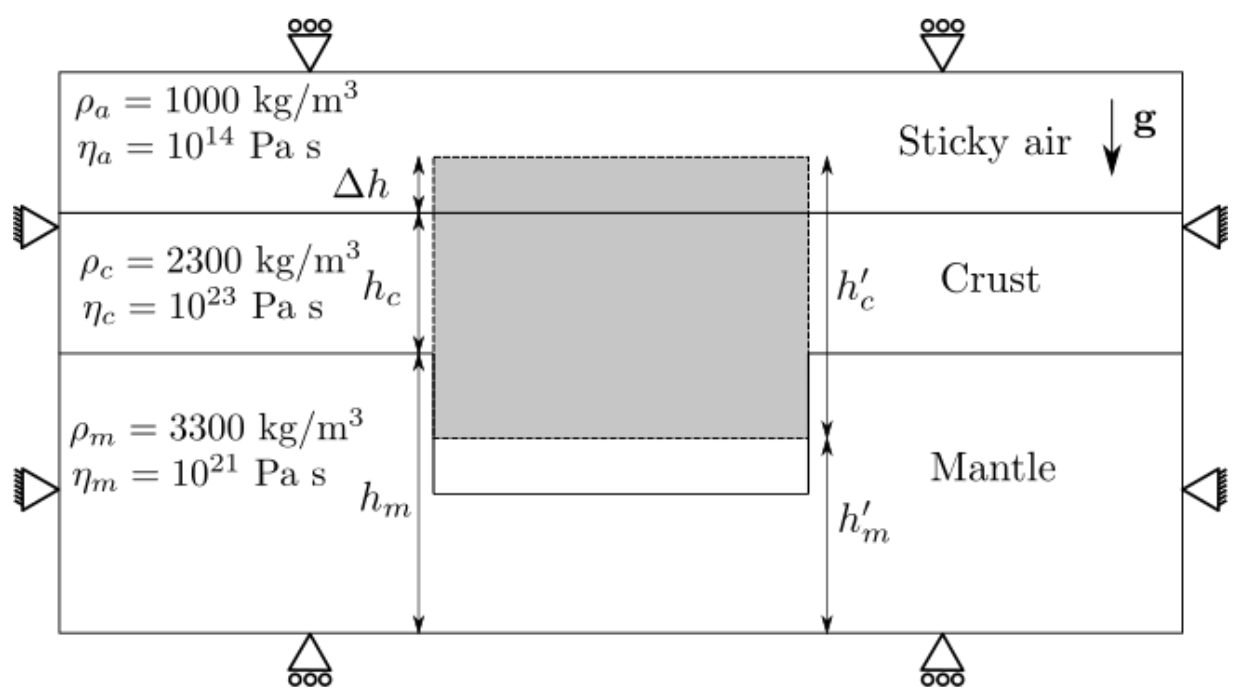
\includegraphics[width=9cm]{python_codes/fieldstone_160/images/setup}\\
{\captionfont Figure by J.C. Afonso. $h_c$ and $h_m$ are the initial thicknesses of the crust and 
mantle. $h_c'$ is the thickness of the thickened crust, and $h_m'$ is the thickness of the 
mantle below the thickened crust at isostatic equilibrium. Drawing not to scale. The gray 
area represents the final position of the tickened crust.}
\end{center}


The thickened crust has a positive buoyancy with respect to the normal crust due
to density difference, whose analytical value is found via a standard isostatic balance (i.e.
equating the mass per unit area of two columns at the compensation level, here taken at
the base of the numerical domain).




On the left or right sides, the lithostatic pressure at the base of the crust is then 
$\rho_{c} g h_{c}=2300*10*20000=460~\si{\mega\pascal}$.
At the base of the model, then the pressure is $450e6+\rho_{m} g h_{m}
=450e6+3300*10*80000=450e6+2640e6=3090~\si{\mega\pascal}$.
In a more abstract way, $P_{bottom}=\rho_c g h_c + \rho_m g h_m$.
In the middle, after the block has moved up and is now in isostatic equilibrium, 
we should have $P_{bottom}=\rho_c g h_c' + \rho_m g h_m'$.
In the end:
\[
P_{bottom}=\rho_c g h_c + \rho_m g h_m = \rho_c g h_c' + \rho_m g h_m'
\]
We can divide both sides by $g$:
\begin{eqnarray}
\rho_c  h_c + \rho_m  h_m &=& \rho_c  h_c' + \rho_m  h_m' \nn\\
\Rightarrow \rho_m h_m'&=& \rho_c(h_c-h_c') + \rho_m h_m  \nn\\
\Rightarrow h_m' &=& h_m-(h_c'-h_c)\frac{\rho_c}{\rho_m} \nn
\end{eqnarray}
Then the dynamic topography is computed as follows:
\begin{eqnarray}
\Delta h 
&=& h_c' + h_m' - h_c - h_m \nn\\
&=& h_c' + h_m -(h_c'-h_c)\frac{\rho_c}{\rho_m} -h_c - h_m \nn\\
&=& h_c'  -(h_c'-h_c)\frac{\rho_c}{\rho_m} -h_c  \nn\\
&=& (h_c'-h_c)  -(h_c'-h_c)\frac{\rho_c}{\rho_m}   \nn\\
&=& (h_c'-h_c) \left(1 -\frac{\rho_c}{\rho_m} \right) 
\end{eqnarray}
Substituting for the parameters of our example, the predicted topography uplift is 
\[
\Delta h = (40000-20000)*(1-2300/3300) \simeq 6060~\si{\meter}
\]


In the \aspect manual we find the following documentation for the 'dynamic topography' post-processor:
``
A postprocessor that computes a measure of dynamic topography based on the stress at the boundary. 
The exact approach works as follows: At each selected boundary, we compute the traction that acts normal to 
the boundary faces using the consistent boundary flux method as described in \textcite{grls87}
From this traction, the dynamic topography is computed using the formula $h=\sigma_n / \rho g$ where $g$
is the norm of the gravity and $\rho$
is the density [of the fluid right below the surface]. 
''

In practice the dynamic topography is then computed as follows: 
\[
h= \frac{\vec{n} \cdot {\bm \sigma}\cdot \vec{n}}{\rho_c g } 
= \frac{\sigma_{yy}}{\rho_c g}
= \frac{-p+\tau_{yy}}{\rho_c g}
\]
where $\vec{n}$ is the normal vector to the surface\footnote{$\vec{t} ={\bm\sigma}\cdot \vec{n}$ 
is the traction on the boundary and then $\vec n \cdot \vec t$ is the component of this traction
along the normal.}. 


\begin{center}
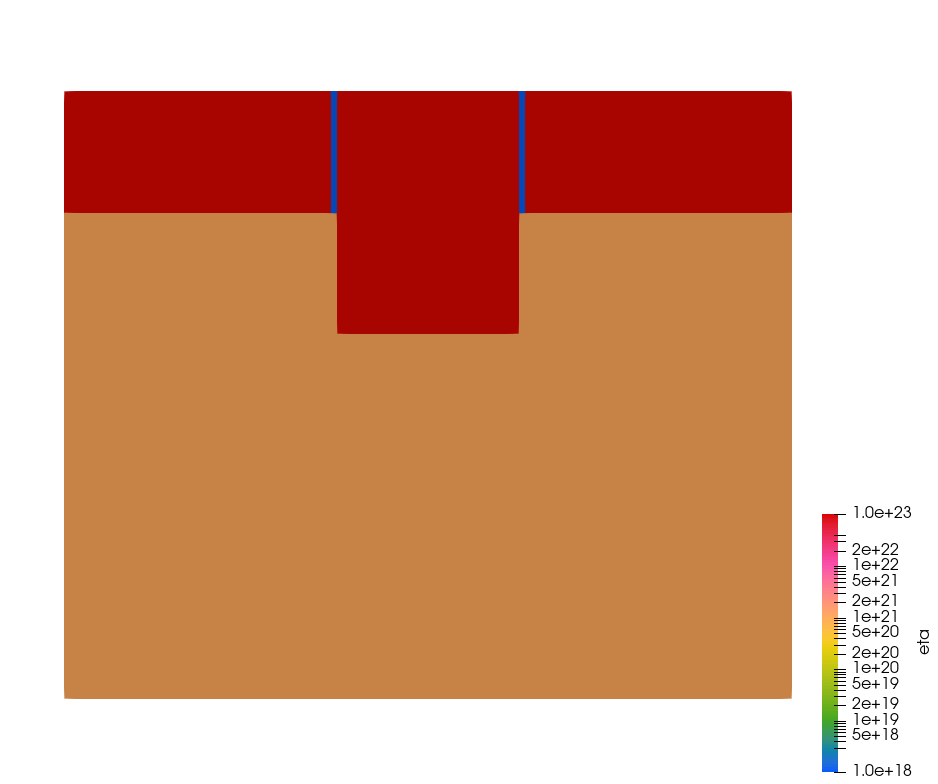
\includegraphics[width=8cm]{python_codes/fieldstone_160/results/eta.png}

\includegraphics[width=8cm]{python_codes/fieldstone_160/results/rho.png}\\
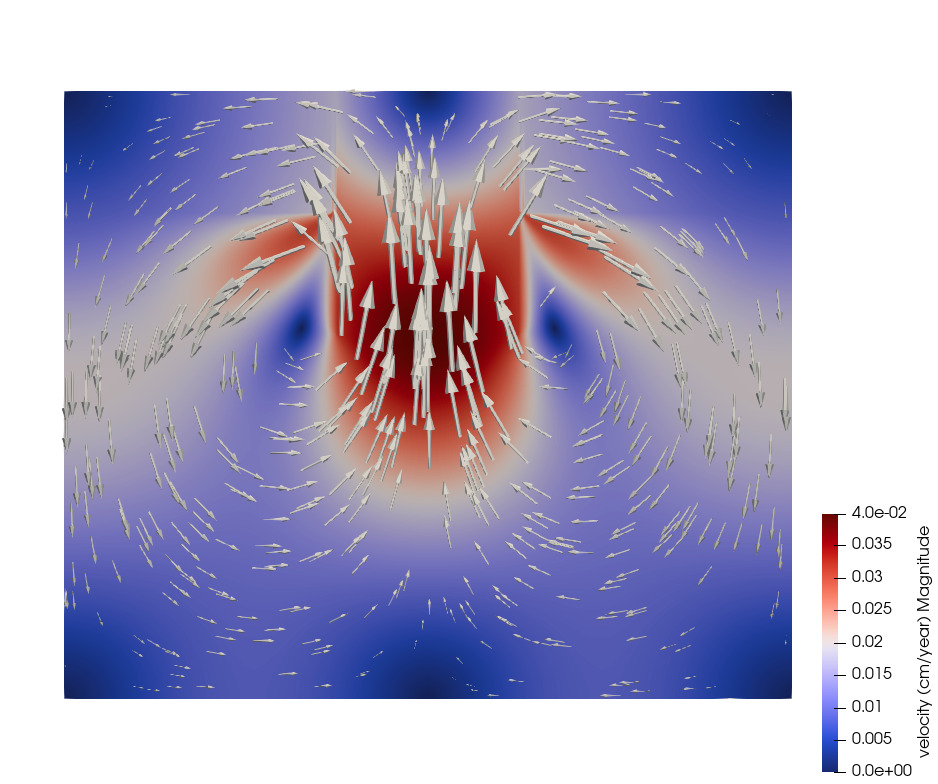
\includegraphics[width=8cm]{python_codes/fieldstone_160/results/vel.png}

\includegraphics[width=8cm]{python_codes/fieldstone_160/results/press.png}\\
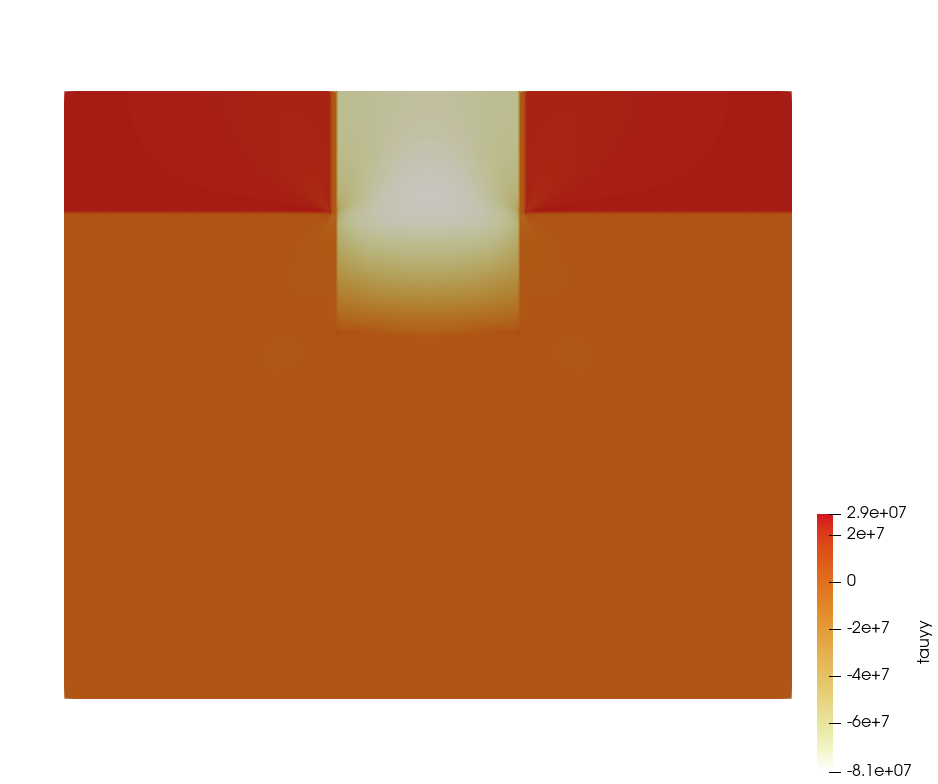
\includegraphics[width=8cm]{python_codes/fieldstone_160/results/tau_yy.png}
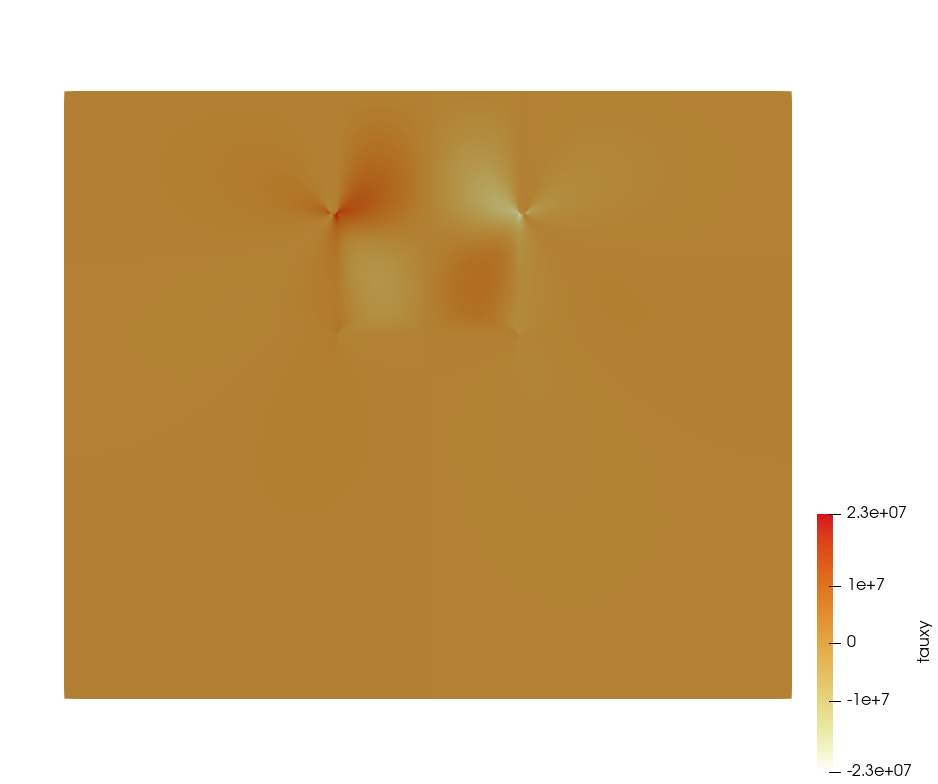
\includegraphics[width=8cm]{python_codes/fieldstone_160/results/tau_xy.png}\\
{\captionfont Results obtained on 240x200 mesh. Top row: viscosity and density fields;
Middle row: velocity and pressure fields; 
Bottom row: $\tau_{yy}$ and $\tau_{xy}$ fields.}
\end{center}



The surface pressure, $yy$ component of deviatoric stress ${\bm \tau}$ 
and dynamic topography are shown in the following plots
\begin{center}
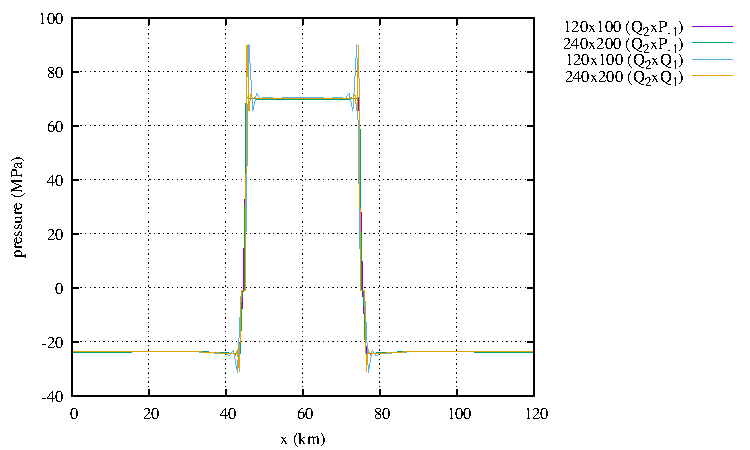
\includegraphics[width=8.5cm]{python_codes/fieldstone_160/results/pressure.pdf}
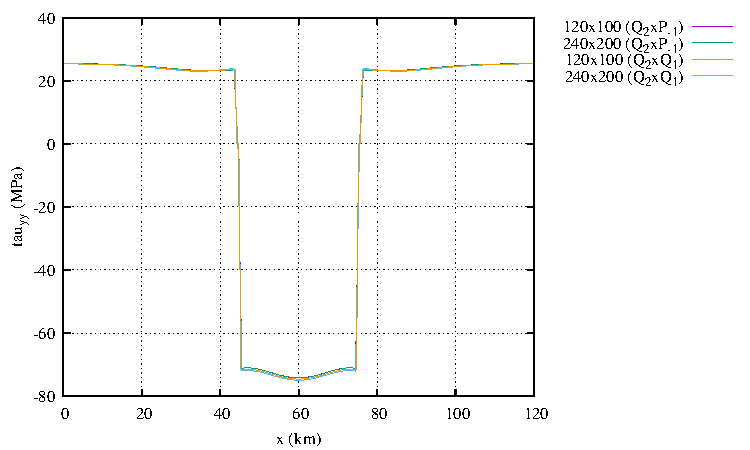
\includegraphics[width=8.5cm]{python_codes/fieldstone_160/results/tau_yy.pdf}\\
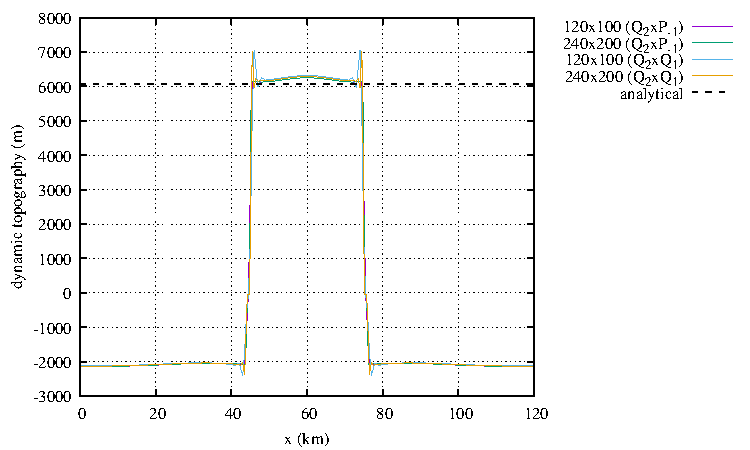
\includegraphics[width=8.5cm]{python_codes/fieldstone_160/results/dyn_topo.pdf}
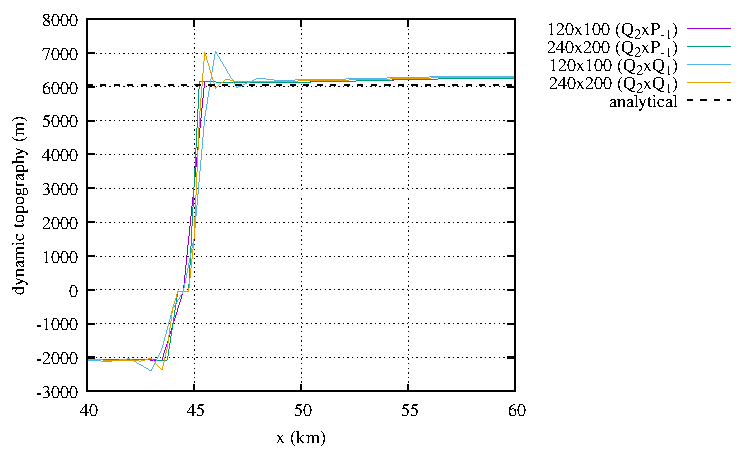
\includegraphics[width=8.5cm]{python_codes/fieldstone_160/results/dyn_topo2.pdf}
\end{center}
We find that the differences between low and high resolution are really small. 
The recovered dynamic topography is very close to the expected analytical value,
but since its accuracy is not improving with resolution this probably means that the 
weak zones and/or the coupling of the keel of the crust with the mantle is 
playing a prominent role.
We also find that the discontinuous pressure element unsurprisingly copes better 
with the element boundary-aligned viscosity jumps, while the continuous pressure 
one yields overshoots on the pressure field.

Let us now investigate the influence of the weak zones viscosity on the 
dynamic topography (zoomed on the important part):
\begin{center}
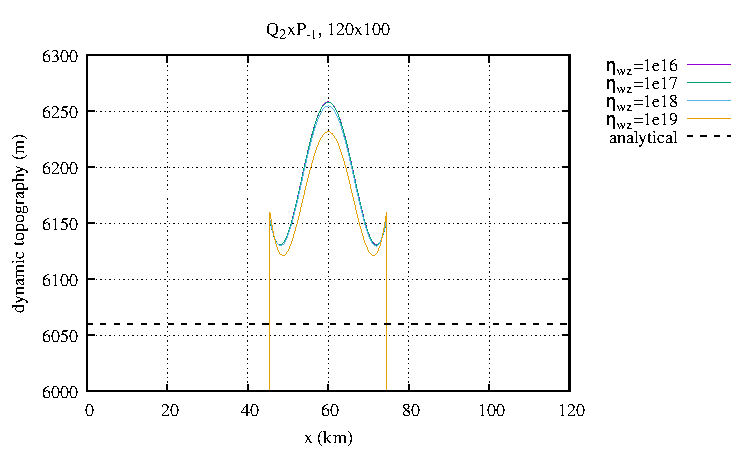
\includegraphics[width=8.5cm]{python_codes/fieldstone_160/results/dyn_topo3a.pdf}
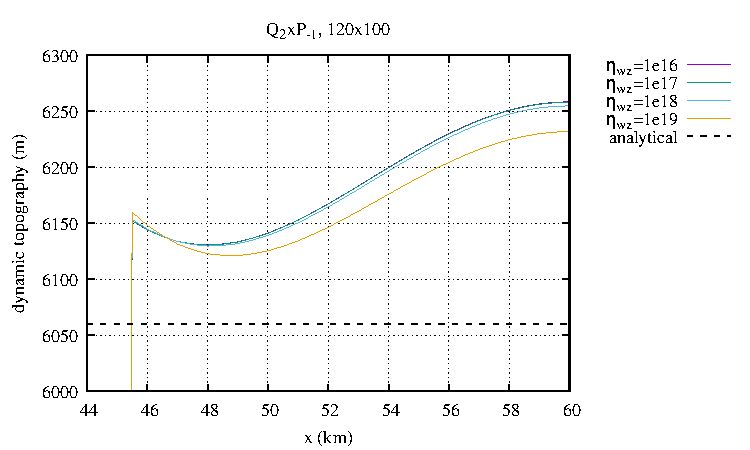
\includegraphics[width=8.5cm]{python_codes/fieldstone_160/results/dyn_topo3b.pdf}
\end{center}
The default value of $\eta_{wz}=10^{18}~\si{\pascal\second}$ is clearly low enough since lower values do not 
yield any visible change. This means that the signal we observe is entirely due
to the geometry of the experiment and/or the coupling crust keel-mantle.

We can now look at the influence of the mantle viscosity (while keeping the 
weak zones at $\eta_{wz}=10^{18}~\si{\pascal\second}$:
\begin{center}
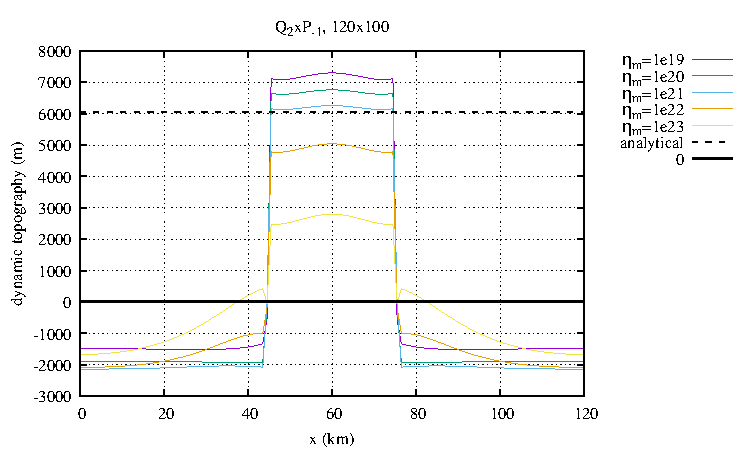
\includegraphics[width=8.5cm]{python_codes/fieldstone_160/results/dyn_topo4a.pdf}
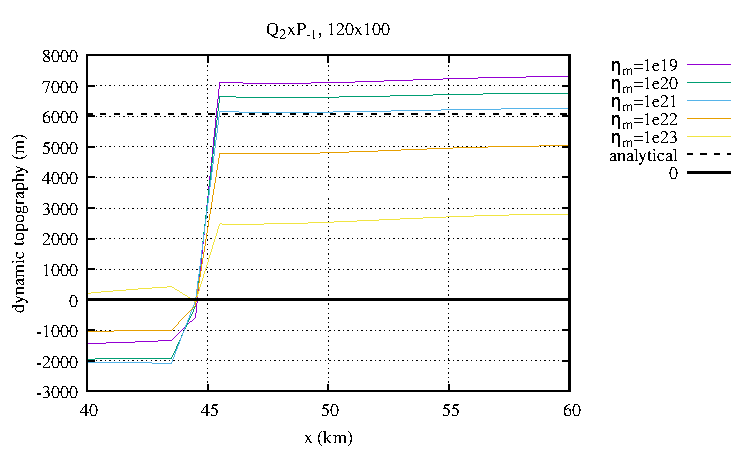
\includegraphics[width=8.5cm]{python_codes/fieldstone_160/results/dyn_topo4b.pdf}
\end{center}
The higher the viscosity of the mantle, the lower the dynamic topography (why?). 
It appears that $\eta_m=10^{21}~\si{\pascal\second}$ yields a dynamic topography
closest to the expected theoretical value.
It is also worth noting that on each side of the block the dynamic topography
is about -2000m.
Looking at the velocity field on the previous page figure, we see that the domain
is such that the positive buoyancy of the block generates a convection cell which 
therefore pulls down the crust on each side of the block.

Let us now investigate the influence of the box geometry (and in particular its 
lateral extent $L_x$ while keeping a $1\times 1$ km resolution).
\begin{center}
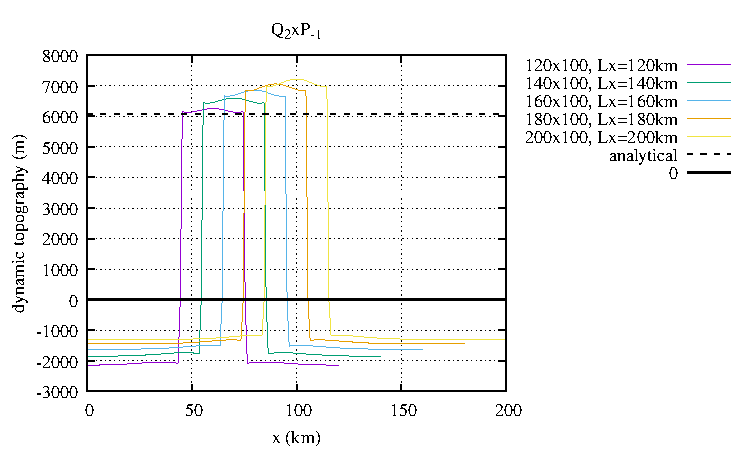
\includegraphics[width=8.5cm]{python_codes/fieldstone_160/results/dyn_topo5.pdf}
\end{center}

In light of all this, let us now prescribe the lithostatic pressure (Neumann boundary conditions)
on the left and right boundaries so as to allow for free in/outflow and hopefully tame the 
return flow. A single node in the middle of the bottom boundary is assigned $u=0$ so as 
to remove the translational nullspace. We recover the following velocity field 
for the default setup:
\begin{center}
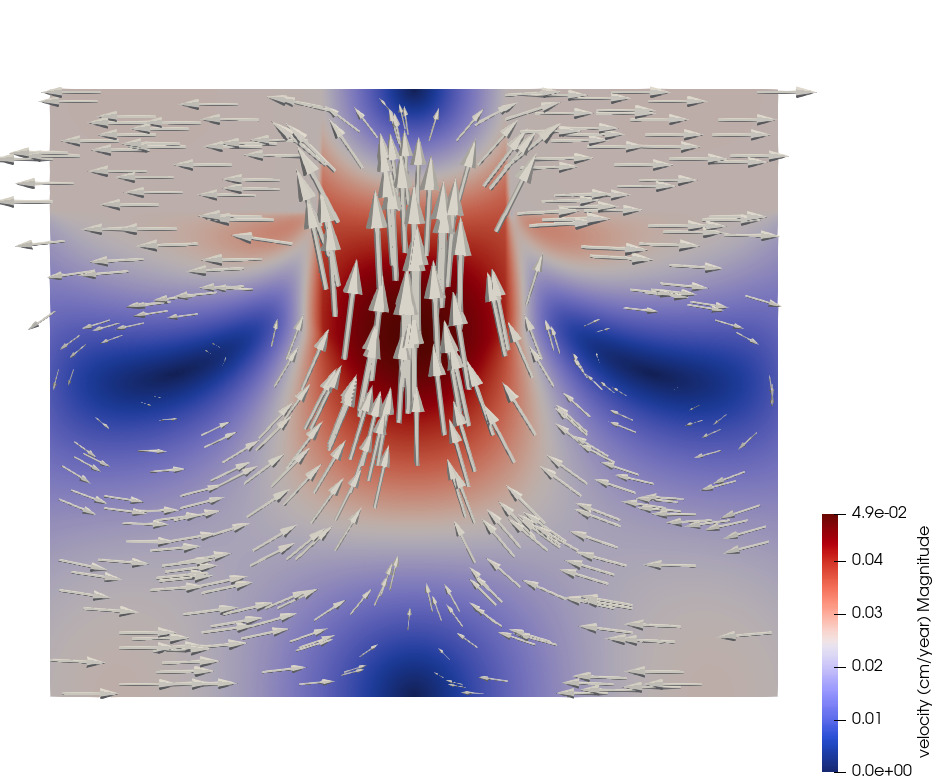
\includegraphics[width=8.5cm]{python_codes/fieldstone_160/results/neumann/velN}
\end{center}
and the dynamic topography varies with $L_x$ as follows:
\begin{center}
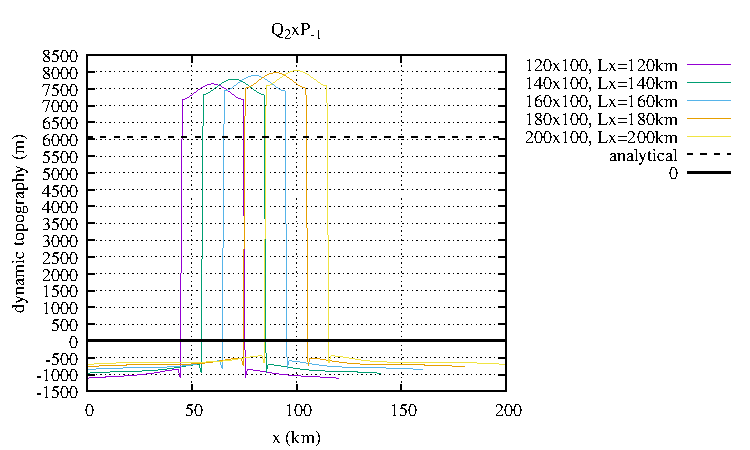
\includegraphics[width=8.5cm]{python_codes/fieldstone_160/results/dyn_topo6.pdf}
\end{center}
We find that the dynamic topography is less dependent on horizontal extent than before
but still increases by about 1000m.

 
In light of all this, I am a bit lost as to what this theoretical value 
stands for. I guess an infinitely long and deep domain? 
My plan is to revisit this with \aspect asap to make sure that these results are correct.





